\section{Experiments}
\label{sec:experiments}

All speedups are baseline time divided by DrainSinkhorn time. OT-stage time is
measured directly or reconstructed by subtracting the paired consumer time from
the encompassing recorded interval. For reconstructed rows, consumer time is
subtracted within each paired timing unit before ratios, intervals, or bootstrap
summaries are formed. Matched component comparisons hold inputs, proposal,
tolerance, verification schedule, two-marginal verifier, and consumer fixed.
Complete-path comparisons use the same packed or vectorized backend in both
arms. When stopping
controllers produce different achieved residuals, the achieved residuals and
consumer-output deviations are reported together.

Accordingly, the reported ratios have two causal roles:
\[
\begin{gathered}
\underbrace{\text{fixed-width}\rightarrow\text{dynamic}}_{\text{release and dynamic compaction}},\\[-1pt]
\underbrace{\text{logical mask}\rightarrow\text{dynamic}}_{\text{width effect}}.
\end{gathered}
\]
Fixed-width/dynamic-compaction measures the net change from a conventional
fixed-width batch to the dynamic-compaction controller; logical-mask/dynamic-compaction
(LM/DC) isolates dynamic width reduction under matched release decisions.
Figure~\ref{fig:main-results-width} reports the measured width-cost curves, and
Table~\ref{tab:main-results-by-width} groups registered effects by initial width. Appendix
Table~\ref{tab:attribution-map} specifies the implementation, timing scope,
and statistical unit of every contrast. Bootstrap intervals on frozen workloads
quantify timing reproducibility conditional on the frozen inputs and execution
configuration. Each contrast is interpreted within its listed campaign and
measurement interval.

\begin{figure*}[!t]
\centering
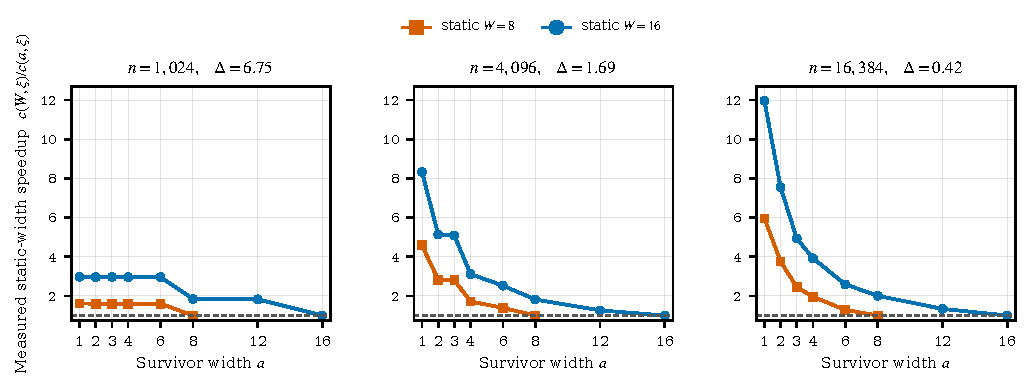
\includegraphics[width=\textwidth]{figures/MAIN_RESULTS_WIDTH_COST.pdf}
\caption{Measured conversion from survivor width to packed-update speedup.
Each curve reports $g_W(a)=c(W,\xi)/c(a,\xi)$ relative to static width
$W\in\{8,16\}$; all panels use the same axes, and shading propagates the
per-width interquartile endpoints from 30 repeats. Panel titles report
$\Delta=b_mN_{\mathrm{SM}}/n$, which determines scheduling-wave quantization.}
\label{fig:main-results-width}
\end{figure*}
\begin{table*}[!t]
\centering
\caption{Registered matched results grouped by initial width. Speedup is
baseline time divided by dynamic-compaction time. Brackets give registered
95\% intervals and parentheses give observed seed or plan ranges. Rows retain
their study-specific timing scopes and are not pooled. Row-level provenance is
recorded in \texttt{support/figure\_materials/MAIN\_RESULTS\_BY\_WIDTH.csv}.}
\label{tab:main-results-by-width}
\scriptsize
\setlength{\tabcolsep}{3.2pt}
\renewcommand{\arraystretch}{1.08}
\begin{tabular}{@{}>{\centering\arraybackslash}p{.035\textwidth}
>{\raggedright\arraybackslash}p{.105\textwidth}
>{\raggedright\arraybackslash}p{.135\textwidth}
>{\raggedright\arraybackslash}p{.105\textwidth}
>{\raggedright\arraybackslash}p{.17\textwidth}
>{\raggedright\arraybackslash}p{.34\textwidth}@{}}
\toprule
$W$ & Campaign & Configuration & Contrast & Speedup & Timing scope and statistical unit \\
\midrule
8 & ImageNet-32 & $n=1024$ & fixed/DC & $1.054\times$ (1.033--1.072) & solver field; 3 training seeds \\
8 & ImageNet-32 & $n=1024$ & fixed/DC & $1.105\times$ (1.079--1.156) & coupling preparation; 3 problem--plan seeds \\
8 & Packer19 & $n=16384$ & LM/DC & $1.5397\times$ [1.5389, 1.5404] & consumer-subtracted OT stage; 24 paired units \\
8 & Packer19 & $n=16384$ & LM/DC & $1.5713\times$ [1.5701, 1.5726] & direct OT stage at $10^{-3}$; 24 paired units \\
8 & MetroPT-3 & $n=16384$, route 3 & fixed/DC & $2.159\times$ & eight-worker complete endpoint; fixed work per worker \\
8 & MetroPT-3 & $n=16384$, route 2 & fixed/DC & $3.110\times$ & eight-worker complete endpoint; fixed work per worker \\
\midrule
16 & ImageNet-32 & $n=4096$, shared anchor & fixed/DC & $1.421\times$ & steady-state critical path; 40 windows \\
16 & ImageNet-32 & $n=4096$, OTT-JAX & fixed/DC & $1.581\times$ & matched 20-update phases; 10 repeats \\
16 & MetroPT-3 & $n=32768$, route 3 & fixed/DC & $1.616\times$ & one-worker endpoint; equal-host geometric mean \\
16 & MetroPT-3 & $n=16384$, two hosts & fixed/DC & $1.7447\times$ [1.7434, 1.7467] & ready-arrays-to-consumer endpoint; 6 host--plan units \\
16 & MetroPT-3 & $n=16384$, four workers & fixed/DC & $1.7455\times$ (1.7453--1.7460) & four-worker makespan; 3 registered plans \\
16 & MetroPT-3 & $n=8192$, route 3 & fixed/DC & $2.316\times$ & one-worker endpoint; equal-host geometric mean \\
\bottomrule
\end{tabular}
\end{table*}


\subsection{Matched release and dynamic compaction}

The matched comparisons begin from conventional fixed-width batched execution.
C82 directly compares the two current MetroPT-3 paths on one host with four
complete-device workers. Dynamic compaction gives
\CMetroCorrectedEndpointSpeedup{} on the ready-arrays-to-consumer endpoint while
problem-update slots fall from \CMetroSlotsStatic{} to \CMetroSlotsActive{}.
All three predeclared execution plans favor dynamic-compaction execution, with a
descriptive range of \CMetroCorrectedEndpointRange{}. The two arms each invoke 16
verifier candidates, evaluate 16 candidates, and launch 32 plan-application
kernels per repeat. The corresponding four-GPU energy ratio is
\CMetroCorrectedEnergyFactor{}.

C66 supplies a separate two-host matched study. Its fixed-width/dynamic-compaction ratio
is $1.744723\times$ on the E2 endpoint and \CMetroRetirementOTSpeedup{} after
subtracting the paired consumer within each host--plan unit. Its six host--plan
units all favor dynamic-compaction execution.

C67 extends the same complete-device design to eight independent workers on two hosts. Its two fixed-per-worker endpoint cells give $3.110\times$ and
$2.159\times$ matched fixed-width/dynamic-compaction speedups while reducing
slots as shown in \cref{tab:c67-global8}. Separate one-worker support-size cells
that pass the frozen gates on both hosts give $2.316\times$ at $n=8192$ and
$1.616\times$ at $n=32768$.

\begin{table}[t]
\centering
\caption{C67 fixed-per-worker execution on eight complete-device workers across
two hosts. Times aggregate the complete consumer endpoint. Slots count
problem updates across workers; energy uses the same endpoint.}
\label{tab:c67-global8}
\scriptsize
\setlength{\tabcolsep}{3pt}
\resizebox{\columnwidth}{!}{%
\begin{tabular}{@{}lrrrrr@{}}
\toprule
Route & Fixed (s) & Dynamic (s) & Slots fixed/dynamic & Time & Energy \\
\midrule
failure-2 & 12.523 & 4.026 & 4736 / 1276 & 3.110$\times$ & 3.437$\times$ \\
failure-3 & 7.999 & 3.705 & 3008 / 1244 & 2.159$\times$ & 2.292$\times$ \\
\bottomrule
\end{tabular}}
\end{table}


In C63, each training step uses a real ImageNet-32 PCA500 feature coupling.
Table~\ref{tab:absolute-ot-times} reports the four solver-phase times. Paired
solver-field fixed-width/dynamic-compaction is $1.054\times$ (observed seed range
$1.033$--$1.072\times$; \cref{tab:c63-solver-pairs}). On the complete fixed-update
training interval, fixed-width/dynamic-compaction is
\CFeatureTrainingActiveOverStatic{} (range
\CFeatureTrainingActiveOverStaticRange{}). C62 separately measures coupling
preparation over three problem-plan seeds, with fixed-width/dynamic-compaction $1.105\times$.
The study that uses one initialization for multiple problems supplies a
non-cold setting: across 40 controlled overlapping-support windows, compacted
execution is $1.421\times$ faster,
reduces slots by 30.62\%, and wins every paired window.

\begin{table*}[t]
\centering
\caption{ImageNet-32 PCA500 feature-space quality after 50k training updates.
Entries are three-seed means for matched fixed-width (Fixed) and dynamically
compacted (Dynamic) execution. Lower is better for all three metrics. The
same three paired training seeds are used throughout the quality evaluation;
the full per-seed measurements and analysis artifacts are available in the
public GitHub repository. These are feature-space metrics, not pixel-space
FID.}
\label{tab:imagenet-quality}
\small
\begin{tabular}{@{}c cc cc cc@{}}
\toprule
& \multicolumn{2}{c}{Curvature} & \multicolumn{2}{c}{Held-out FM MSE} & \multicolumn{2}{c}{Projected Fr\'echet} \\
NFE & Fixed & Dynamic & Fixed & Dynamic & Fixed & Dynamic \\
\midrule
4  & 5.4524 & 5.4448 & 1.07854 & 1.07859 & 1.2967 & 1.2886 \\
8  & 2.8388 & 2.8356 & 1.07854 & 1.07859 & 1.5286 & 1.5224 \\
16 & 1.4546 & 1.4528 & 1.07854 & 1.07859 & 1.8182 & 1.8136 \\
\bottomrule
\end{tabular}
\end{table*}


The numerical quality results use the same three paired training seeds at NFE
4, 8, and 16. The full per-seed measurements and analysis artifacts are
available in the public GitHub repository at
\url{https://github.com/cis-aconiticacid/DrainSinkhorn}.
The evaluation measures the ImageNet-32 PCA500 feature-space OT-FM endpoint.

\subsection{Measured conversion from width to kernel time}

We measure the width-cost term in \cref{eq:time-difference} by calling the same
packed Triton update at fixed problem size and varying only the width.
\Cref{fig:main-results-width} normalizes the measured medians as
$g_W(a)=c(W,\xi)/c(a,\xi)$ for static widths $W=8$ and $16$, using the common
survivor-width coordinates $a\in\{1,2,3,4,6,8,12,16\}$. For a realized
survivor width $A_k$, the corresponding summand in
\cref{eq:time-difference} is
$c(W,\xi_k)[1-g_W(A_k)^{-1}]$. The panel value
$\Delta=b_mN_{\mathrm{SM}}/n$ predicts the plateau scale: conversion is
quantized at $n=1024$ ($\Delta=6.75$), becomes finer at $n=4096$
($\Delta=1.69$), and is near continuous at $n=16384$ ($\Delta=0.42$).

The diagnostic isolates the packed update, so it estimates one component of
$c_k(a,\xi_k)$ rather than the complete executor. Its $n=1024,W=8$ shape is
consistent with the modest C63 solver-field ratio: after the survivor width
enters the $A\leq6$ region, further lane removal changes slot count more than
packed-update time. The $n=16384$ response provides the corresponding hardware
condition for the larger MetroPT-3 dynamic-compaction gains; the matched C82 endpoint
then measures the complete net effect, including control and consumer work.

\paragraph{Transfer across backend families.}
The OTT-JAX and PyKeOps rows test the execution principle with independent
implementations. OTT-JAX execution that processes only the remaining problems in each
fixed phase is \COTTNativeActiveSpeedup{} faster than native OTT-JAX on real
ImageNet-32 at $W=16$; its matched fixed-width/dynamic-compaction control assigns
\COTTStaticActiveSpeedup{} to removing completed problems only at phase
boundaries and then rebucketing the survivors. On real
A2D2 LiDAR, the PyKeOps compacted path is \CKeopsLiDARActiveSpeedup{} faster than
sequential carry at $W=8$. A real ImageNet-32 PyKeOps cell remains positive at
\CKeopsImageNetActiveSpeedup{}. The tiled-log implementation reaches $n=65536$
without materializing per-problem cost tensors and supplies the measured capacity
boundary.

Independent OTT-JAX and PyKeOps realizations are summarized in
\cref{tab:ot-cross-backend}.

\subsection{Packer19 stopping and execution Pareto}

The two-host EXP-PACKER19 campaign evaluates residual tolerances
$10^{-4}$, $3\times10^{-4}$, $10^{-3}$, $3\times10^{-3}$, and $10^{-2}$
without aggregating across tolerances. All arms use the same two-marginal
verifier and residual tolerance, and the same tight-reference consumer output.

\begin{figure*}[t]
\centering
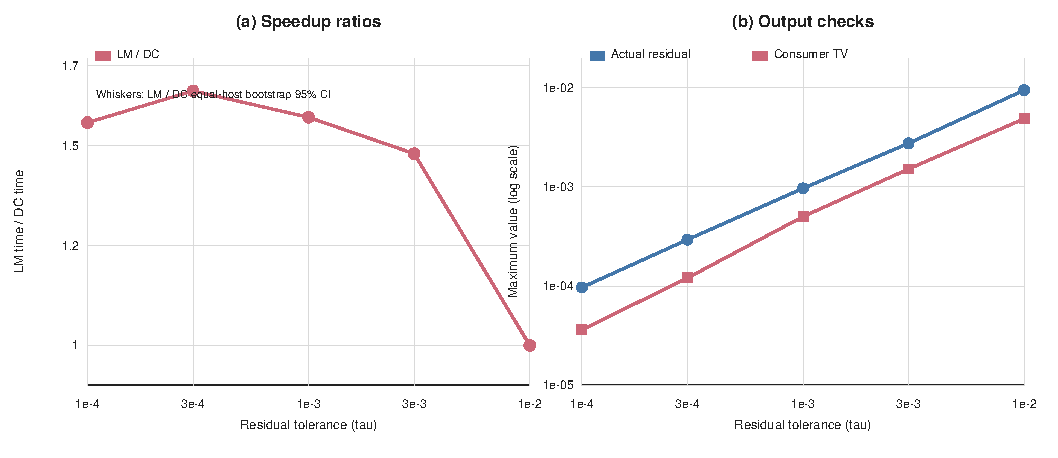
\includegraphics[width=\textwidth]{figures/PACKER19_STOPPING_METRICS.pdf}
\caption{Two-host Packer19 stopping--execution results under a common
two-marginal verifier and residual tolerance. Panel (a) shows the LM/DC speedup ratio across
the five tolerances. Whiskers are the equal-host
stratified bootstrap 95\% intervals for LM/DC. Panel (b) shows maximum actual residual
and maximum consumer TV on a logarithmic scale. Each point summarizes 24
paired units; consumer TV measures differences in outputs against the tight
reference.}
\label{fig:packer-stopping-metrics}
\end{figure*}

Dynamic compaction improves over logical masking by \CPackerCompactionRange{}
at $10^{-4}$ through $3\times10^{-3}$. At $10^{-2}$,
all eight problems first pass at update 8, so there is no removable padding
and LM/DC is neutral at \CPackerNeutralCompaction{} (95\% CI
\CPackerNeutralCompactionCI{}). These valid contrasts characterize
EXP-PACKER19's complete and logical-mask paths; the earlier C80-LM controls and
phase costs are reported
separately in \cref{tab:c80-attribution,tab:phase-costs}.

All registered endpoint quality checks pass.

\subsection{Matched component attribution}

\paragraph{Effects of release and dynamic compaction.}
C82 gives \CMetroCorrectedEndpointSpeedup{} on the matched MetroPT-3 E2 endpoint;
C66 gives \CMetroRetirementOTSpeedup{} on its separately measured E1 OT stage.
In the C63 ImageNet-32
four-arm training ablation, dynamic compaction adds
\CFeatureTrainingActiveOverStatic{} over fixed-width batching across three seeds
(range \CFeatureTrainingActiveOverStaticRange{}). This is an E3 endpoint
attribution; the $1.054\times$ C63 solver-field comparison is reported
separately in \cref{tab:absolute-ot-times,tab:c63-solver-pairs}.

C80 and C80-LM use the same Packer19 single-cell transition workload on two hosts, each with four A100-SXM4-80GB GPUs. Three frozen method orders
produce 24 paired host--order--GPU units. Each unit uses warmup-excluded repeat
medians, the same input, packed-kernel source tree, $10^{-3}$ stopping tolerance, and transition
consumer.

\begin{table}[t]
\centering
\caption{MetroPT-3 grouping intervention on one fixed real task multiset. For
offline every-cycle iteration numbers $q_s$ within a window,
$H_q=\operatorname{sd}(q_s)/\operatorname{mean}(q_s)$ and
padding is $W\max_s q_s/\sum_s q_s-1$. Dynamic slots is the ratio of dynamic to
static candidate-iteration slots. The displayed values aggregate over windows;
timing repeats stabilize each condition and are not independent datasets.}
\label{tab:m3-grouping}
\scriptsize
\setlength{\tabcolsep}{3pt}
\begin{tabular}{@{}lcccc@{}}
\toprule
Grouping & $H_q$ & Padding & Dynamic slots & Fixed/dynamic \\
\midrule
heterogeneous & 0.236 & 0.236 & 0.802 & 1.217$\times$ \\
homogeneous & 0.127 & 0.110 & 0.892 & 1.105$\times$ \\
random 1 & 0.254 & 0.293 & 0.776 & 1.258$\times$ \\
random 2 & 0.264 & 0.270 & 0.789 & 1.235$\times$ \\
random 3 & 0.260 & 0.279 & 0.764 & 1.271$\times$ \\
\bottomrule
\end{tabular}
\end{table}


\paragraph{Verifier and screen ablation}
The controls expose distinct work. Batched evaluation of the two-marginal
verifier and the preliminary screen using the current marginals reduce OT-stage
time under matched paths. Each C80 ratio subtracts its paired consumer time
before forming the contrast.

We replay all \CPackerShadowNegatives{} screen-negative events and evaluate
each with the two-marginal verifier, finding
\CPackerShadowMissedReady{} already-releasable lanes. The maximum difference
between the preliminary screen and verifier row residual is
\CPackerScreenDiscrepancy{}. Every emitted plan passes the two-marginal
verifier at $10^{-3}$.

\paragraph{Logical masking versus dynamic compaction.}
In C80-LM, logical masking is neutral because the packed kernel retains width
eight. Dynamic compaction reduces the observed width, removes 100 of 256 problem-update slots, and yields \CPackerCompactionOTSpeedup{} OT-stage acceleration with
interval \CPackerCompactionOTRange{}. All 24 paired units favor dynamic compaction.
Across the 24 host--order--GPU unit medians, endpoint energy falls from 879.9 to
688.1 J, while compacted buffers raise peak allocated memory from 80.8 to
106.9 MiB.

\subsection{Operating regime: heterogeneity and width}

M3 holds the set of 32 real MetroPT problems fixed; only their grouping into
windows changes. Offline every-cycle iteration numbers $q_t$ define the
grouping, while the verifier-derived iteration numbers $n_t$ measure executed
work. Oracle homogeneous grouping minimizes variation in the required
iteration numbers within each window. Heterogeneous and random groupings
increase the area between the static rectangle and the survival curve defined
by $n_t$. The
matched fixed-width/dynamic-compaction ratio grows from
\CMThreeHomogeneousRetirementSpeedup{} to
\CMThreeHeterogeneousRetirementSpeedup{} and 1.235--1.271$\times$ on random
layouts.

\begin{table}[t]
\centering
\caption{Packer19 single-variable attribution under one frozen input and
release contract. Every row reports OT-stage time from a paired comparison
after subtracting consumer time,
so the component effects share one measurement boundary.}
\label{tab:c80-attribution}
\scriptsize
\setlength{\tabcolsep}{2.6pt}
\resizebox{\columnwidth}{!}{%
\begin{tabular}{@{}lllll@{}}
\toprule
Change & Matched contrast & Scope & Ratio & Evidence \\
\midrule
Batched verification & serial / batched verifier & OT stage & 1.133$\times$ & 24/24 wins \\
Preliminary current-marginal screen & verifier only / preliminary screen & OT stage & 1.105$\times$ & 24/24 wins \\
Logical freeze & fixed / logical mask & OT stage & 1.000$\times$ & 95\% CI [0.9998, 1.0003] \\
Dynamic compaction & logical mask / dynamic compaction & OT stage & \CPackerCompactionOTSpeedup{} & 95\% CI \CPackerCompactionOTRange{} \\
\bottomrule
\end{tabular}}
\vspace{2pt}

{\scriptsize The batched verification and preliminary current-marginal-screen
rows have 24/24 paired wins; no
separate E1 bootstrap interval is registered for those two contrasts.}
\end{table}


\paragraph{Independent finite-precision stress test.}
C10 measures decision behavior on 84 near-threshold problems and 16 runtime
attacks over 1/2/4/8 GPUs. Relative to independent FP64 replay, raw FP32 and
TF32 each disagree on three accept decisions; an outward-bound guard followed
by FP64 escalation has zero disagreements in these 100 cases. This guarded
configuration is evaluated separately from the timed applications.

\paragraph{Timed applications and independent-worker scale-out.}
The timed packed Triton path uses the precision supported by the backend and the
two-marginal verifier. All emitted plans meet both recorded marginal-residual
bounds, and every
endpoint passes its registered output or quality check. C67 assigns complete
windows to independent GPU workers. Four workers achieve
3.965--3.979$\times$ fixed-per-worker throughput scaling on held-out MetroPT
routes, with no Sinkhorn collective between workers; the eight-worker matched
endpoint decomposition appears in \cref{tab:c67-global8}.

